\documentclass[boxes]{gsypset}

% Info for header
\mailbox{}
\initials{}
\collaborators{}
\class{Math 60}
\assignment{HW 11}
\duedate{June 1, 2016}
\problemlist{6.2.\{R10, 13, 15\}, 6.3.\{1, 3, 4, R7, 25, R26, 33\}}

\usepackage{caption}

\begin{document}
	\begin{problem}[6.2.13]
		Evaluate $\oint_C (x^4y^5 - 2y)\dx{x} + (3x + x^5y^4)\dx{y}$, 
		where $C$ is the oriented curve pictured in Figure 6.29.
		
		\begin{center}
			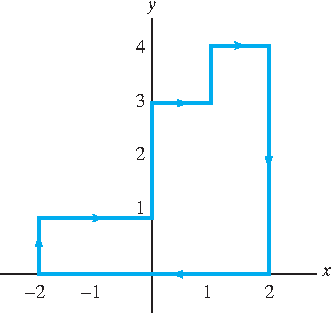
\includegraphics{img/6_2_13}
			\renewcommand{\thefigure}{6.29}
			\captionof{figure}{The oriented curve $C$ of Exercise 13.}
		\end{center}
	\end{problem}
	\begin{solution}
		
	\end{solution}
	
	\begin{problem}[6.2.15]
		\begin{subproblems}
			\subproblem Sketch the curve given parametrically by $\mathbf{x}(t) = \bm{1-t^2, & t^3-t}$.
				\begin{solution}
					
				\end{solution}
			\subproblem Find the area inside the closed loop of the curve.
				\begin{solution}
					
				\end{solution}
		\end{subproblems}
	\end{problem}
	
	\begin{problem}[6.3.1]
		Consider the line integral $\int_C z^2 \dx{x} + 2y \dx{y} + xz \dx{z}$.
		\begin{subproblems}
			\subproblem 
				Evaluate this integral, where $C$ is the line segment from $(0, 0, 0)$ to $(1, 1, 1)$.
				\begin{solution}
					
				\end{solution}
			\subproblem 
				Evaluate this integral, where $C$ is the path from $(0, 0, 0)$ to $(1, 1, 1)$ 
				parametrized by $\mathbf{x}(t) = \bm{t, & t^2, & t^3}$, $0 \leq t \leq 1$.
				\begin{solution}
					
				\end{solution}
			\subproblem 
				Is the vector field $\mathbf{F} = \bm{z^2, & 2y, & xz}$ conservative? Why or why not?
				\begin{solution}
					
				\end{solution}
		\end{subproblems}
	\end{problem}
	
	\begin{problem}[6.3.3]
		Determine whether the vector field $\mathbf{F} = \bm{e^{x+y}, & e^{xy}}$ is conservative.
		If it is, find a scalar potential function for $\mathbf{F}$.
	\end{problem}
	\begin{solution}
		
	\end{solution}
	
	\begin{problem}[6.3.4]
		Determine whether the vector field $\mathbf{F} = \bm{2x \sin y, & x^2 \cos y}$ is conservative.
		If it is, find a scalar potential function for $\mathbf{F}$.
	\end{problem}
	\begin{solution}
		
	\end{solution}
	
	\begin{problem}[6.3.25]
		Let $\mathbf{F} = \bm{x^2, & \cos y \sin z, & \sin y \cos z}$.
		\begin{subproblems}
			\subproblem 
				Show that $\mathbf{F}$ is conservative and 
				find a scalar potential function $f$ for $\mathbf{F}$.
				\begin{solution}
					
				\end{solution}
			\subproblem 
				Evaluate $\int_\mathbf{x}\mathbf{F} \cdot \mathrm{d}\mathbf{s}$
				along the path $\mathbf{x}: [0,1] \to \mathbb{R}^3$,
				$\mathbf{x}(t) = \bm{t^2 + 1, & e^t, & e^{2t}}$.
				\begin{solution}
					
				\end{solution}
		\end{subproblems}
	\end{problem}
	
	\begin{problem}[6.3.33]
		\begin{subproblems}
			\subproblem 
				Determine where the vector field
				\[
					\mathbf{F} = \bm{\dfrac{x + xy^2}{y^2} & -\dfrac{x^2 + 1}{y^3}}
				\]
				is conservative.
				\begin{solution}
					
				\end{solution}
			\subproblem Determine a scalar potential for $\mathbf{F}$.
				\begin{solution}
					
				\end{solution}
			\subproblem 
				Find the work done by $\mathbf{F}$ in moving a particle along the parabolic curve
				$y = 1 + x - x^2$ from $(0, 1)$ to $(1, 1)$.
				\begin{solution}
					
				\end{solution}
		\end{subproblems}
	\end{problem}
\end{document}